%%%%%%%%%%%%%%%%%%%%%%%%%%%%%%%%%%%%%%%%%
% Using a0poster Portrait Poster 1.0 from LaTeX Template
% The a0poster class was created by:
% Gerlinde Kettl and Matthias Weiser (tex@kettl.de)
%%%%%%%%%%%%%%%%%%%%%%%%%%%%%%%%%%%%%%%%%

%----------------------------------------------------------------------------------------
%	PACKAGES AND OTHER DOCUMENT CONFIGURATIONS
%----------------------------------------------------------------------------------------

\documentclass[a0,portrait]{a0poster}

\usepackage{multicol} % This is so we can have multiple columns of text side-by-side
\columnsep=100pt % This is the amount of white space between the columns in the poster
\columnseprule=3pt % This is the thickness of the black line between the columns in the poster

\usepackage[svgnames]{xcolor} % Specify colors by their 'svgnames', for a full list of all colors available see here: http://www.latextemplates.com/svgnames-colors

% \usepackage{times} % Use the times font
%\usepackage{palatino} % Uncomment to use the Palatino font

\usepackage{graphicx} % Required for including images
% \graphicspath{{figures/}} % Location of the graphics files
\usepackage{booktabs} % Top and bottom rules for table
\usepackage[font=small,labelfont=bf]{caption} % Required for specifying captions to tables and figures
\usepackage{amsfonts, amsmath, amsthm, amssymb} % For math fonts, symbols and environments
\usepackage{wrapfig} % Allows wrapping text around tables and figures

\usepackage[ukrainian,russian]{babel}
\usepackage[utf8]{inputenc}
\usepackage{fontenc}

\usepackage{ulem}

\usepackage[unicode,pdfusetitle, bookmarks=true, bookmarksnumbered=true,bookmarksopen=true,bookmarksopenlevel=1]{hyperref}
\hypersetup{backref,colorlinks=true,linkcolor=blue,citecolor=green,bookmarks=false}


% \usepackage{fancyhdr}
% \pagestyle{fancy}
% \fancyhead[C]{Заседание N$\sqrt(2)$, 12-ого октября 2013, в комнате 401 Института математики (ул. Терещенковская, 3)  в 14.00}

\newtheorem{theor}{Теорема}[section]
\newtheorem{defin}{Определение}[section]
\newtheorem{example}{Пример}[section]
\newtheorem{exe}{Упражнение}[section]
\newtheorem{stat}{Утверждение}[section]
\newtheorem{lemma}{Лемма}[section]
\newtheorem{stat2}{Соглашение}[section]


% % % % % % % % % % % % % % % % % % % 
% From: Physics, Topology, Logic and Computation: A Rosetta Stone


%famous categories
\newcommand{\Cob}{\mathrm{Cob}}
\newcommand{\Hilb}{\mathrm{Hilb}}
\newcommand{\Set}{\mathrm{Set}}
\newcommand{\Fin}{\mathrm{Fin}}
\newcommand{\Cat}{{\rm Cat}}
\newcommand{\Tang}{{\rm Tang}}
\newcommand{\Lie}{{\rm Lie}}
\newcommand{\Grp}{{\rm Grp}}
\newcommand{\CommRing}{{\rm CommRing}}
\newcommand{\Diff}{{\rm Diff}}
\newcommand{\Rep}{{\rm Rep}}
\newcommand{\Vect}{{\rm Vect}}
\newcommand{\Braid}{{\rm Braid}}
\newcommand{\Rel}{{\rm Rel}}
\newcommand{\Super}{{\rm Super}}
\newcommand{\Th}{\mathrm{Th}}

%arrows
\newcommand{\maps}{\colon}
\newcommand{\iso}{\cong}
\newcommand{\isoto}{\xrightarrow{\sim}}
\newcommand{\To}{\Rightarrow}
% \newcommand{\xrightarrow}[1]{\stackrel{#1}{\rightarrow}}
% \newcommand{\implies}{\quad \Rightarrow \quad}

%homs
\newcommand{\lHom}{\vdash}
\newcommand{\lhom}{\multimap}
\newcommand{\rhom}{\leftspoon}
\renewcommand{\hom}{{\rm hom}}
\newcommand{\HOM}[2]{{#1 \lhom #2}}

%products
\newcommand{\tensor}{\otimes}
\newcommand{\x}{\times}
\newcommand{\OTIMES}{{\boldmath$\otimes$ \,}}
\newcommand{\TENSOR}{{\boldmath$\hat{\otimes}$ \,}}
\newcommand{\CIRC}{{\boldmath$\circ$ \,}}
\newcommand{\LAMBDA}{{\boldmath$\lambda$ \,}}
\newcommand{\ab}[1]{\langle #1 \rangle} % "angle brackets"

%morphisms, rules, constants
\newcommand{\id}{{\rm i}}
\newcommand{\Id}{{\rm id}}
\newcommand{\ev}{{\rm ev}}
\newcommand{\coev}{{\rm coev}}
\newcommand{\eval}{{\rm eval}}
\newcommand{\app}{{\rm app}}
\newcommand{\assoc}{{\rm assoc}}
\newcommand{\unassoc}{{\rm unassoc}}
\newcommand{\braid}{{\rm braid}}
\newcommand{\Left}{{\rm left}}
\newcommand{\Right}{{\rm right}}
\newcommand{\unright}{{\rm unright}}
\newcommand{\unleft}{{\rm unleft}}
\newcommand{\Tensor}{{\rm tensor}}
\newcommand{\swap}{{\rm swap}}
\newcommand{\term}{{\rm term}}
\newcommand{\cp}{{\rm cp}}
\newcommand{\vp}{{\rm vp}}
\newcommand{\cut}{{\circ}}
\newcommand{\op}{{\rm op}}   
\newcommand{\name}[1]{\ulcorner \! #1 \! \urcorner}
\newcommand{\inv}{${}^{-1}$}

%data types and programs
\newcommand{\plus}{{\rm plus}}
\newcommand{\Times}{{\rm times}}
\newcommand{\double}{{\rm double}}
\newcommand{\increment}{{\rm increment}}
\newcommand{\Day}{{\rm day}}
\newcommand{\Tuesday}{{\rm Tuesday}}
\newcommand{\integer}{{\rm integer}}
\newcommand{\duplicate}{{\rm duplicate}}
\newcommand{\curry}{{\rm curry}}
\newcommand{\uncurry}{{\rm uncurry}}
\newcommand{\compose}{{\rm compose}}
% % % % % % % % % % % % % % % % % % % 
%    Q-circuit version 2
%    Copyright (C) 2004  Steve Flammia & Bryan Eastin
%    Last modified on: 9/16/2011
%
%    This program is free software; you can redistribute it and/or modify
%    it under the terms of the GNU General Public License as published by
%    the Free Software Foundation; either version 2 of the License, or
%    (at your option) any later version.
%
%    This program is distributed in the hope that it will be useful,
%    but WITHOUT ANY WARRANTY; without even the implied warranty of
%    MERCHANTABILITY or FITNESS FOR A PARTICULAR PURPOSE.  See the
%    GNU General Public License for more details.
%
%    You should have received a copy of the GNU General Public License
%    along with this program; if not, write to the Free Software
%    Foundation, Inc., 59 Temple Place, Suite 330, Boston, MA  02111-1307  USA

% Thanks to the Xy-pic guys, Kristoffer H Rose, Ross Moore, and Daniel Müllner,
% for their help in making Qcircuit work with Xy-pic version 3.8.  
% Thanks also to Dave Clader, Andrew Childs, Rafael Possignolo, Tyson Williams,
% Sergio Boixo, Cris Moore, Jonas Anderson, and Stephan Mertens for helping us test 
% and/or develop the new version.

\usepackage{xy}
\xyoption{matrix}
\xyoption{frame}
\xyoption{arrow}
\xyoption{arc}

\usepackage{ifpdf}
\ifpdf
\else
\PackageWarningNoLine{Qcircuit}{Qcircuit is loading in Postscript mode.  The Xy-pic options ps and dvips will be loaded.  If you wish to use other Postscript drivers for Xy-pic, you must modify the code in Qcircuit.tex}
%    The following options load the drivers most commonly required to
%    get proper Postscript output from Xy-pic.  Should these fail to work,
%    try replacing the following two lines with some of the other options
%    given in the Xy-pic reference manual.
\xyoption{ps}
\xyoption{dvips}
\fi

% The following resets Xy-pic matrix alignment to the pre-3.8 default, as
% required by Qcircuit.
\entrymodifiers={!C\entrybox}

\newcommand{\bra}[1]{{\left\langle{#1}\right\vert}}
\newcommand{\ket}[1]{{\left\vert{#1}\right\rangle}}
    % Defines Dirac notation. %7/5/07 added extra braces so that the commands will work in subscripts.
\newcommand{\qw}[1][-1]{\ar @{-} [0,#1]}
    % Defines a wire that connects horizontally.  By default it connects to the object on the left of the current object.
    % WARNING: Wire commands must appear after the gate in any given entry.
\newcommand{\qwx}[1][-1]{\ar @{-} [#1,0]}
    % Defines a wire that connects vertically.  By default it connects to the object above the current object.
    % WARNING: Wire commands must appear after the gate in any given entry.
\newcommand{\cw}[1][-1]{\ar @{=} [0,#1]}
    % Defines a classical wire that connects horizontally.  By default it connects to the object on the left of the current object.
    % WARNING: Wire commands must appear after the gate in any given entry.
\newcommand{\cwx}[1][-1]{\ar @{=} [#1,0]}
    % Defines a classical wire that connects vertically.  By default it connects to the object above the current object.
    % WARNING: Wire commands must appear after the gate in any given entry.
\newcommand{\gate}[1]{*+<.6em>{#1} \POS ="i","i"+UR;"i"+UL **\dir{-};"i"+DL **\dir{-};"i"+DR **\dir{-};"i"+UR **\dir{-},"i" \qw}
    % Boxes the argument, making a gate.
\newcommand{\meter}{*=<1.8em,1.4em>{\xy ="j","j"-<.778em,.322em>;{"j"+<.778em,-.322em> \ellipse ur,_{}},"j"-<0em,.4em>;p+<.5em,.9em> **\dir{-},"j"+<2.2em,2.2em>*{},"j"-<2.2em,2.2em>*{} \endxy} \POS ="i","i"+UR;"i"+UL **\dir{-};"i"+DL **\dir{-};"i"+DR **\dir{-};"i"+UR **\dir{-},"i" \qw}
    % Inserts a measurement meter.
    % In case you're wondering, the constants .778em and .322em specify
    % one quarter of a circle with radius 1.1em.
    % The points added at + and - <2.2em,2.2em> are there to strech the
    % canvas, ensuring that the size is unaffected by erratic spacing issues
    % with the arc.
\newcommand{\measure}[1]{*+[F-:<.9em>]{#1} \qw}
    % Inserts a measurement bubble with user defined text.
\newcommand{\measuretab}[1]{*{\xy*+<.6em>{#1}="e";"e"+UL;"e"+UR **\dir{-};"e"+DR **\dir{-};"e"+DL **\dir{-};"e"+LC-<.5em,0em> **\dir{-};"e"+UL **\dir{-} \endxy} \qw}
    % Inserts a measurement tab with user defined text.
\newcommand{\measureD}[1]{*{\xy*+=<0em,.1em>{#1}="e";"e"+UR+<0em,.25em>;"e"+UL+<-.5em,.25em> **\dir{-};"e"+DL+<-.5em,-.25em> **\dir{-};"e"+DR+<0em,-.25em> **\dir{-};{"e"+UR+<0em,.25em>\ellipse^{}};"e"+C:,+(0,1)*{} \endxy} \qw}
    % Inserts a D-shaped measurement gate with user defined text.
\newcommand{\multimeasure}[2]{*+<1em,.9em>{\hphantom{#2}} \qw \POS[0,0].[#1,0];p !C *{#2},p \drop\frm<.9em>{-}}
    % Draws a multiple qubit measurement bubble starting at the current position and spanning #1 additional gates below.
    % #2 gives the label for the gate.
    % You must use an argument of the same width as #2 in \ghost for the wires to connect properly on the lower lines.
\newcommand{\multimeasureD}[2]{*+<1em,.9em>{\hphantom{#2}} \POS [0,0]="i",[0,0].[#1,0]="e",!C *{#2},"e"+UR-<.8em,0em>;"e"+UL **\dir{-};"e"+DL **\dir{-};"e"+DR+<-.8em,0em> **\dir{-};{"e"+DR+<0em,.8em>\ellipse^{}};"e"+UR+<0em,-.8em> **\dir{-};{"e"+UR-<.8em,0em>\ellipse^{}},"i" \qw}
    % Draws a multiple qubit D-shaped measurement gate starting at the current position and spanning #1 additional gates below.
    % #2 gives the label for the gate.
    % You must use an argument of the same width as #2 in \ghost for the wires to connect properly on the lower lines.
\newcommand{\control}{*!<0em,.025em>-=-<.2em>{\bullet}}
    % Inserts an unconnected control.
\newcommand{\controlo}{*+<.01em>{\xy -<.095em>*\xycircle<.19em>{} \endxy}}
    % Inserts a unconnected control-on-0.
\newcommand{\ctrl}[1]{\control \qwx[#1] \qw}
    % Inserts a control and connects it to the object #1 wires below.
\newcommand{\ctrlo}[1]{\controlo \qwx[#1] \qw}
    % Inserts a control-on-0 and connects it to the object #1 wires below.
\newcommand{\targ}{*+<.02em,.02em>{\xy ="i","i"-<.39em,0em>;"i"+<.39em,0em> **\dir{-}, "i"-<0em,.39em>;"i"+<0em,.39em> **\dir{-},"i"*\xycircle<.4em>{} \endxy} \qw}
    % Inserts a CNOT target.
\newcommand{\qswap}{*=<0em>{\times} \qw}
    % Inserts half a swap gate.
    % Must be connected to the other swap with \qwx.
\newcommand{\multigate}[2]{*+<1em,.9em>{\hphantom{#2}} \POS [0,0]="i",[0,0].[#1,0]="e",!C *{#2},"e"+UR;"e"+UL **\dir{-};"e"+DL **\dir{-};"e"+DR **\dir{-};"e"+UR **\dir{-},"i" \qw}
    % Draws a multiple qubit gate starting at the current position and spanning #1 additional gates below.
    % #2 gives the label for the gate.
    % You must use an argument of the same width as #2 in \ghost for the wires to connect properly on the lower lines.
\newcommand{\ghost}[1]{*+<1em,.9em>{\hphantom{#1}} \qw}
    % Leaves space for \multigate on wires other than the one on which \multigate appears.  Without this command wires will cross your gate.
    % #1 should match the second argument in the corresponding \multigate.
\newcommand{\push}[1]{*{#1}}
    % Inserts #1, overriding the default that causes entries to have zero size.  This command takes the place of a gate.
    % Like a gate, it must precede any wire commands.
    % \push is useful for forcing columns apart.
    % NOTE: It might be useful to know that a gate is about 1.3 times the height of its contents.  I.e. \gate{M} is 1.3em tall.
    % WARNING: \push must appear before any wire commands and may not appear in an entry with a gate or label.
\newcommand{\gategroup}[6]{\POS"#1,#2"."#3,#2"."#1,#4"."#3,#4"!C*+<#5>\frm{#6}}
    % Constructs a box or bracket enclosing the square block spanning rows #1-#3 and columns=#2-#4.
    % The block is given a margin #5/2, so #5 should be a valid length.
    % #6 can take the following arguments -- or . or _\} or ^\} or \{ or \} or _) or ^) or ( or ) where the first two options yield dashed and
    % dotted boxes respectively, and the last eight options yield bottom, top, left, and right braces of the curly or normal variety.  See the Xy-pic reference manual for more options.
    % \gategroup can appear at the end of any gate entry, but it's good form to pick either the last entry or one of the corner gates.
    % BUG: \gategroup uses the four corner gates to determine the size of the bounding box.  Other gates may stick out of that box.  See \prop.

\newcommand{\rstick}[1]{*!L!<-.5em,0em>=<0em>{#1}}
    % Centers the left side of #1 in the cell.  Intended for lining up wire labels.  Note that non-gates have default size zero.
\newcommand{\lstick}[1]{*!R!<.5em,0em>=<0em>{#1}}
    % Centers the right side of #1 in the cell.  Intended for lining up wire labels.  Note that non-gates have default size zero.
\newcommand{\ustick}[1]{*!D!<0em,-.5em>=<0em>{#1}}
    % Centers the bottom of #1 in the cell.  Intended for lining up wire labels.  Note that non-gates have default size zero.
\newcommand{\dstick}[1]{*!U!<0em,.5em>=<0em>{#1}}
    % Centers the top of #1 in the cell.  Intended for lining up wire labels.  Note that non-gates have default size zero.
\newcommand{\Qcircuit}{\xymatrix @*=<0em>}
    % Defines \Qcircuit as an \xymatrix with entries of default size 0em.
\newcommand{\link}[2]{\ar @{-} [#1,#2]}
    % Draws a wire or connecting line to the element #1 rows down and #2 columns forward.
\newcommand{\pureghost}[1]{*+<1em,.9em>{\hphantom{#1}}}
    % Same as \ghost except it omits the wire leading to the left. 



\begin{document}

%----------------------------------------------------------------------------------------
%	POSTER HEADER 
%----------------------------------------------------------------------------------------

% The header is divided into two boxes:
% The first is 75% wide and houses the title, subtitle, names, university/organization and contact information
% The second is 25% wide and houses a logo for your university/organization or a photo of you
% The widths of these boxes can be easily edited to accommodate your content as you see fit

\begin{minipage}[b]{0.75\linewidth}
\veryHuge \color{NavyBlue} \textbf{$\mathcal{P}\neq\mathcal{NP}$ и физическая реальность} \color{Black}\\ 
\Huge\textit{О применении поля SU(2) к задачам теории графов}\\[2cm] % Subtitle
\huge \textbf{Андрей Ширай}\\[0.5cm] % Author(s)
\huge School of Sciences,\\
   Miskatonic University\\[0.4cm] % University/organization
\Large \texttt{shiray.and@gmail.com} \\
\end{minipage}
%
\begin{minipage}[b]{0.25\linewidth}
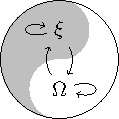
\includegraphics[width=20cm]{../ccs_logo.pdf}\\
\end{minipage}
Заседание \textnumero $\sqrt{2}$, 12-ого октября 2013, в комнате 401 Института математики (ул. Терещенковская, 3)  в 14.00
\vspace{1cm} % A bit of extra whitespace between the header and poster content

%----------------------------------------------------------------------------------------

\begin{multicols}{2} % This is how many columns your poster will be broken into, a portrait poster is generally split into 2 columns

%----------------------------------------------------------------------------------------
%	ABSTRACT
%----------------------------------------------------------------------------------------

\color{Navy} % Navy color for the abstract

\begin{abstract}
Доказательство того, что $\mathcal{P}\neq\mathcal{NP}$ является одной из ключевых проблем современной Теоретической Информатики и Математики. Сомнений в том, что $\mathcal{P}\neq\mathcal{NP}$ (почти) нет, и этому есть не только интуитивно-исторические(ну раз так долго не смогли доказать, что равны, то значит неравны) и интуитивно-математические(схлопывание иерархий классов сложности выгледит подозрительно маловероятным), но и объективные физические сведетельства. Мы можем поставить вопрос равности классов $\mathcal{P}$ и $\mathcal{NP}$ в физической формулировке и свести это злополучное неравенство к физическим постулатам(конечность с, второе начало т/д), которые многократно проверены эксперементально и вполне надежны. Вот такая \textit{эксперементальная математика}.


\end{abstract}

%----------------------------------------------------------------------------------------
%	OBJECTIVES
%----------------------------------------------------------------------------------------

\color{SaddleBrown} % SaddleBrown color for the introduction

\section*{План}

\begin{enumerate}
\item Физика -- это процессы, Информатика -- это процессы
\item Расширенный тезис Тьюринга-Черча
\item Термодинамика алгоритмических процессов
\item Алгоритм Гровера
\item Оптимальность алгоритма Гровера
\item Нелинейные теории КМ
\item Неподвижные точки и путешествия во времени
\item Физика и Информатика с позиции Теории Категорий 
\end{enumerate}

\color{Black} % Black color for the rest of the content
%----------------------------------------------------------------------------------------
%	MATERIALS AND METHODS
%----------------------------------------------------------------------------------------

\section{Физика -- это процессы, Информатика -- это процессы}
\subsection{Физика и Информатика с позиции Теории Категорий}

\begin{center}
 


% \begin{wraptable}{l}{12cm} % Left or right alignment is specified in the first bracket, the width of the table is in the second
\begin{tabular}{l l l}
\toprule
\textbf{Теория категорий} & \textbf{Физика} & \textbf{Теория вычислений}\\
\midrule
Объект $X$       &
Гильбертово пространство $X$  &
Тип данных $X$
\\
\hline
Морфизм &
Оператор &
Программа  \\
$f\maps X \to Y$ &
$f\maps X \to Y$ &
$f \maps X \to Y$
\\
\hline
Тензорное произведение  &
Гильбертово пространство    &
 Произведение 
\\
объектов: &
объединённой системы: &
типов данных: 
\\
$X \tensor Y$ &
$X \tensor Y$ &
$X \tensor Y$ \\

\bottomrule
\end{tabular}
\label{analogy_detailed}
\captionof{table}{\color{Green} The Rosetta Stone}
% \end{wraptable}
\end{center}
% \begin{center}
% \begin{table}
% 
% \begin{tabular}{c|c|c|c|c}
% \hline
% \textbf{Теория категорий} & \textbf{Физика} &  \textbf{Теория вычислений}
% \\
% \hline
% Объект $X$       &
% Гильбертово пространство $X$  &
% Тип данных $X$
% \\
% \hline
% Морфизм &
% Оператор &
% Программа  \\
% $f\maps X \to Y$ &
% $f\maps X \to Y$ &
% $f \maps X \to Y$
% \\
% \hline
% Тензорное произведение  &
% Гильбертово пространство    &
%  Произведение 
% \\
% объектов: &
% объединённой системы: &
% типов данных: 
% \\
% $X \tensor Y$ &
% $X \tensor Y$ &
% $X \tensor Y$
% 
% \end{tabular}
% \caption{The Rosetta Stone}
% \label{analogy_detailed}
% 
% \end{table}
% \end{center}


\subsection{Расширенный тезис Тьюринга-Черча}
\begin{stat}
\label{ct1}
Любая эффективно вычислимая функция может быть эффективно вычислена Машинй Тьюринга
\end{stat}
 \begin{stat}
 \label{ct2}
Любая эффективно вычислимая функция может быть эффективно вычислена Вероятносной МТ

\end{stat}
\begin{stat}
\label{ct3}
Любая эффективно вычислимая функция может быть эффективно вычислена Квантовой МТ

\end{stat}

Какой вариант правильный -- мы не знаем. Важным для нас есть тот момент, что \textit{эффективно вычислимая функция} -- это чисто физическое понятие, точно так же, как и \textit{вычислимая функция} в Тезиче Тьюринга-Черча. Поэтому их можно \textit{эксперементально} проверить! Есть физическая система и есть алгоритм для расчета ее эволюции? Ок, Тезис Тьюринга-Черча верен. Есть физическая система(квантовая) и мы не можем ее проверить на классическом компьюторе? Значит утверждение \ref{ct1} неверно. И т.д.


\subsection{Термодинамика алгоритмических процессов}
Исторически теория информации пошла из термодинамики и статфизики. Непосредственный перенос термодинамических соображений на алгоритмы возможен:
\[
p = \frac{1}{Z} e^{-\beta E(x) -\gamma V(x) - \delta N(x)}
\]
Распределение Гибса со статсуммой: $Z = \sum_{x \in X} e^{-\beta E(x) -\gamma V(x) - \delta N(x)}$
Но! Полученная ``термодинамика'' будет нефизична, так как статсумма невычислима! \footnote{В часности, при $\beta = 0$,
$\gamma = \ln 2$, $\delta = 0$:  $Z = \Omega$ --константа Хатина  }

%----------------------------------------------------------------------------------------
%	RESULTS 
%----------------------------------------------------------------------------------------

\section{Алгоритм Гровера}
\subsection{Квантовая информатика одной табличной}
\begin{center}
\begin{tabular}{c|c}
Стохастика & ``Кванты'' \\ 
% \hline
% \midrule
$ \begin{pmatrix}
s_{11} & \dots &s_{1n}\\ 
\vdots & \ddots & \vdots \\ 
s_{n1} & \dots & s_{nn}
\end{pmatrix}
\begin{pmatrix}
p_1\\ 
\vdots \\ 
p_n
\end{pmatrix}
=
\begin{pmatrix}
q_1\\ 
\vdots \\ 
q_n
\end{pmatrix}$ &
$ \begin{pmatrix}
u_{11} & \dots & u_{1n}\\ 
\vdots & \ddots & \vdots \\ 
u_{n1} & \dots & u_{nn}
\end{pmatrix}
\begin{pmatrix}
\alpha_1\\ 
\vdots \\ 
\alpha_n
\end{pmatrix}
=
\begin{pmatrix}
\beta_1\\ 
\vdots \\ 
\beta_n
\end{pmatrix}$ \\
$ p_i \geq 0, \sum_{i=1}^{n} p_i =1 $ & $ \alpha \in \mathbb{C},  \sum_{i=1}^{n}\left \| \alpha_i \right \|^2 =1  $
\end{tabular}
\end{center}
\subsection{Алгоритм Гровера}

\begin{align*}
 \Qcircuit @C=1em @R=.7em {
                   &         &                      &                         &                      & \ustick{\text{Оператор Гровера G:}} \\
  \lstick{\ket{0}} & /^n \qw & \gate{H^{\otimes n}} & \multigate{1}{O} & \gate{H^{\otimes n}} & \gate{2 \ket{\psi}\bra{\psi} - I_n}         & \gate{H^{\otimes n}} & \qw & \cdots & & \meter & \cw \\
  \lstick{\ket{1}} & \qw     & \gate{H}             & \ghost{O}        & \qw                  & \qw                                       & \qw                  & \qw & \cdots & \\
                   &         &                      &                         &                      & \dstick{\text{Выполняется $O(\sqrt{N})$ раз}}
  \gategroup{2}{5}{2}{7}{.7em}{^\}}
  \gategroup{2}{4}{3}{10}{.7em}{_\}}
 }
\end{align*}
\vspace{1cm}


Сначала формируют равномернe суперпозицию всех состояний: $\operatorname{H}^{\otimes n}\ket{0} = \frac{1}{\sqrt{N}}\sum_x\ket{x}$. Чуть дальше будет обозначать для краткости равномерную суперпозицию как $\ket{\psi}$ Потом последовательно применяется оператор Гровера: 
\begin{enumerate}
 \item К входу применяется оракул $O$: $\ket{x} \to (-1)^{f(x)} \ket{x} $ Т.е. это единичная матрица, где на месте ответов стоят -1. \footnote{Очевидно, что $O^2=I$, так что унитарность сохраняется.}
 \item Опять преобразование Адамара $\operatorname{H}^{\otimes n}$
 \item Условный сдвиг фазы: $\ket{x} \to -(-1)^{\delta_{0x}\ket{x}}$, этой операции соответствует унитарный оператор $\ket{0}\bra{0}-I$.
%  Это тоже унитарная операция: $(\frac{2}{N} - 1)^2 + (N-1)(\frac{2}{N})^2 = \frac{4}{N^2} - \frac{4}{N} + 1 + \frac{4}{N} - \frac{4}{N^2} = 1$ 
 \item Опять преобразование Адамара $\operatorname{H}^{\otimes n}$
\end{enumerate}
\[
 G =  (\ket{\psi}\bra{\psi}-I)O
\]
Физический смысл оператора G довольно простост -- это вращение в двухмерном пространстве, порождаемом вектором $\ket{\psi}$ и ветором-решением. Мы можем переписать $\ket{\psi}$, как:
\[
 \ket{\psi} = \sqrt{\frac{N-M}{N}} \ket{\alpha} + \sqrt{\frac{M}{N}}\ket{\beta}=\cos{\frac{\theta}{2}}\ket{\alpha} + \sin{\frac{\theta}{2}}\ket{\beta}
\]
,где $\ket{\alpha}=\frac{1}{\sqrt{N-M}}\sum_{\neg f(x)}\ket{x}$ и $\ket{\beta}=\frac{1}{\sqrt{M}}\sum_{f(x)}\ket{x}$

\begin{center}\vspace{1cm}
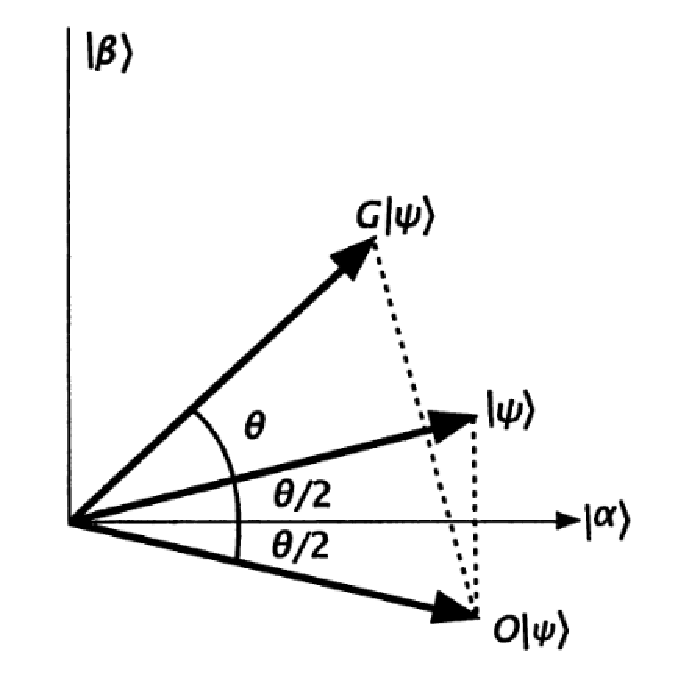
\includegraphics[scale=1]{grvr.pdf}
\captionof{figure}{\color{Green} Геометрическая интерпритация алгоритма Гровера}
\end{center}\vspace{1cm}
\[
 G\ket{\psi} = \cos{\frac{3\theta}{2}}\ket{\alpha} + \sin{\frac{3\theta}{2}}\ket{\beta}
\]
\[
 G^k \ket{\psi} = \cos{\frac{(2k+1)\theta}{2}}\ket{\alpha} + \sin{\frac{(2k+1)\theta}{2}}\ket{\beta}
\]
И необходимое количество итераций:
\[
 R = \lfloor \arccos{\frac{\sqrt{M/N}}{\theta}} \rfloor \stackrel{M \leq N/2}{=} \lfloor \frac{\pi}{4} \sqrt{\frac{N}{M}} \rfloor
\]

\subsection{Оптимальность алгоритма Гровера}
\begin{theor}
 Алгоритм Гровера -- оптимальный
\end{theor}
Идея доказательства состоит в оценке $D_k$ -- меры отклонения оракулом после $k$ вызовов. Она растет не быстрее, чем $O(k^2)$ и имеет порядок $\Omega(N)$, откуда будет следовать, что необходимо не меньше  $\Omega(\sqrt{N})$ обращений к оракулу. 
\[
 O(\sqrt{N}) \wedge \Omega(\sqrt{N}) \Rightarrow \Theta(\sqrt{N})
\]

\subsection{Нелинейные теории КМ и прочее фричество}
\begin{enumerate}
 \item Линейность квантовой механики $\rightarrow$ Предел Гровера $\sqrt{N}$
\item Нелинейная КМ передает сигналы быстрее с и  решает $\mathcal{\#P}$-полные проблемы за полиномиальное время! Ура!
\item ... попутно экспоненциально размножая ошибку. \#\$\^\%\&*!
\item Скрытые параметры? Предел Гровера улучшается с $N^\frac{1}{2}$ до $N^\frac{1}{3}$ -- поиск по ``историям'' траекторий частичек
\item Зеноновские вычисления и всякие прочие супертьюринговые вычисления  накрываются по достижении планковской длины.  
\end{enumerate}

\section{Неподвижные точки и путешествия во времени}
\subsection{Неподвижные точки}
\begin{defin}
 \textbf{Неподвижной точкой} некоторой функции $f$ называется значение $x$ такое, что $f(x) = x$.
\end{defin}

\begin{defin}
 \textbf{Комбинатор неподвижной точки} —- функция высшего порядка, которая вычисляет неподвижную точку заданной функции:
\[
 f (FIX(f))  = FIX (f)
\]
\end{defin}

\begin{example}
  \[
 Y := \lambda\ f. (\lambda\ x . f\  (x \  x)) (\lambda\ x . f\  (x \  x))
\]
\begin{align*}
 Y f = (\lambda\ f.(\lambda\ x.f\  (x\  x)) (\lambda\ x.f\  (x\  x))) f = \\
 = (\lambda\ x.f\  (x\  x)) (\lambda\ x.f\  (x\  x)) =  \\
=  f((\lambda\ x.f\  (x\  x)) (\lambda\ x.f\  (x\  x))) = \\
 =  f(Y f) 
\end{align*}
\end{example}

\begin{example} \textbf{Факториал, ``функциональный'' вариант:}
\[
 F = \lambda\ f\ n. if\ n=0\ then\ 1\ else\ n * f(n-1)
\]
\[
 fact = Y F
\]

Функция F соответствует одному шагу рекурсии, комбинатор неподвижной точки реализует (рекурсивное) вычисление
\end{example}

\subsection{Time travel for fun and profit}

Для начала рассмотрим упрощенную стохастическую, а не квантовую систему
\begin{itemize}
 \item  Убил дедушку: $\begin{bmatrix}
1 \\
0 
\end{bmatrix}$
\item Не убил деда: $\begin{bmatrix}
0 \\
1 
\end{bmatrix}$
\item 
\[
\begin{bmatrix}
0 & 1\\
1 & 0
\end{bmatrix}  \vec{v} = \vec{v} 
\]

\item Неподвижная точка: 
\[
 \vec{v}= \frac{1}{2}\begin{bmatrix}
1 \\
1 
\end{bmatrix}
\]

\end{itemize}
А теперь переходим от стохастических матриц к матрицам плотности:
\begin{equation}
\label{soper}
\rho_{CTC} =S(\rho_{CTC} )
\end{equation} 
S -- некий супероператор: $\rho \xrightarrow{S} \sum_i E_i \rho E_i^\dag, \sum_i E_i^\dag E_i = I$. Супероператор S не является произвольным. Для того, что бы уравнение \ref{soper} имело смысл результатом его применения должна быть матрица плотности.


Основной результат Дойча состоит в том, что:
\begin{theor}
  Уравнение $\rho_{CTC} =S(\rho_{CTC} )$ имеет неподвижную точку(т.е. оно всегда разрешимо)
\end{theor}

Идея времяпутешественных вычислений состоит в использовани временной петли аналогично оракулу.
\begin{center}\vspace{1cm}
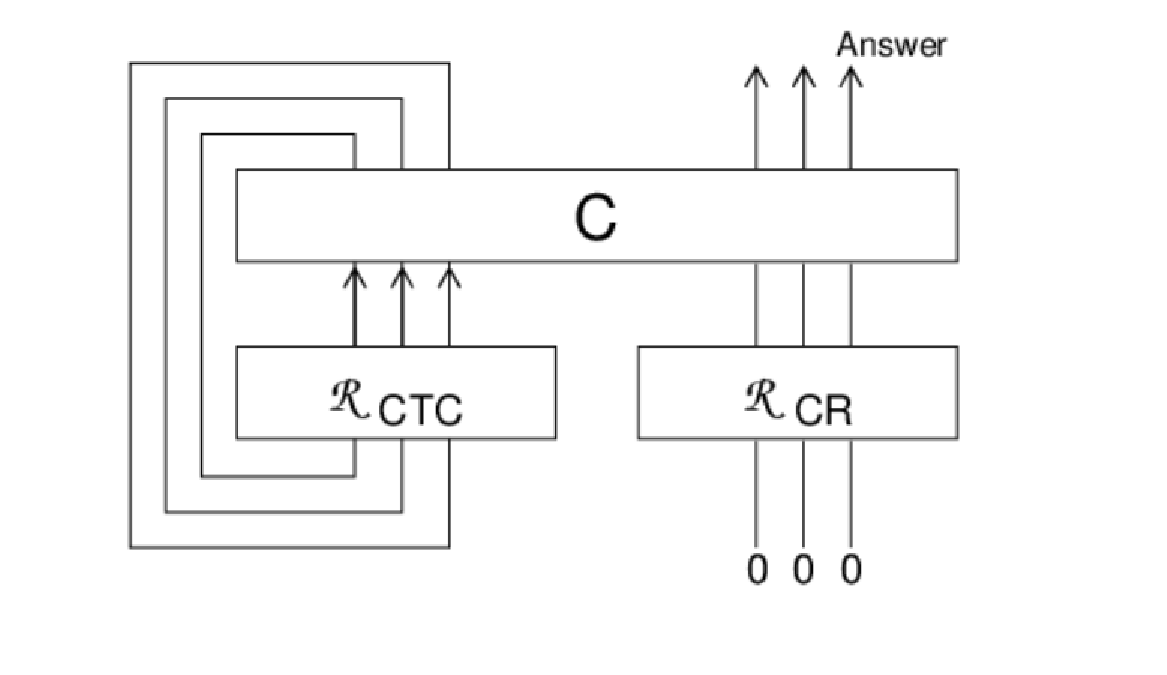
\includegraphics[scale=1]{ctcfig.pdf}
\captionof{figure}{\color{Green} Time travel for fun and profit}
\end{center}\vspace{1cm}

%----------------------------------------------------------------------------------------
%	CONCLUSIONS
%----------------------------------------------------------------------------------------






%----------------------------------------------------------------------------------------
%	FORTHCOMING RESEARCH
%----------------------------------------------------------------------------------------
% \color{Navy}
% \section{Открытые проблемы}
% 
% Vivamus molestie, risus tempor vehicula mattis, libero arcu volutpat purus, sed blandit sem nibh eget turpis. Maecenas rutrum dui blandit lorem vulputate gravida. Praesent venenatis mi vel lorem tempor at varius diam sagittis. Nam eu leo id turpis interdum luctus a sed augue. Nam tellus.
% 
% \color{Black} % Set the color back to Black for the rest of the content
 %----------------------------------------------------------------------------------------
%	REFERENCES
%----------------------------------------------------------------------------------------

\nocite{*} % Print all references regardless of whether they were cited in the poster or not
\bibliographystyle{plain} % Plain referencing style
\bibliography{bib} % Use the example bibliography file sample.bib

%----------------------------------------------------------------------------------------
%	ACKNOWLEDGEMENTS
%----------------------------------------------------------------------------------------

\section*{Благодарности}

Я благодарен Николаю Вовчанскому и Василию Кузнецову за живительный пинок и идею организации семинара.

%----------------------------------------------------------------------------------------

\end{multicols}
\end{document}